
%\section{Calibration and Validation}
\section{Validation}
\label{sec:validation}

%
% meshed vanes are 24x more expensive
%

The previous sections briefly outlined the physical phenomenon under
consideration, the mathematical models proposed to simulate this phenomenon,
and the numerical solution of these models 
for a variety of system configurations and scenarios. 

Before these simulations can be used as a tool to evaluate proposed system 
designs, it is necessary to validate that the model accurately represents 
the real system. 

%% However, for our simulations to be useful for prediction, we
%% need to evaluate models against experimental data so
%% as to ensure that the entire formulation accurately reflects reality. 
Here, the validation of the computational models
against existing experimental data and high fidelity simulations is 
discussed.\todo{need to describe the experiment}

%
% experimental challenges
%

The general system configuration is depicted
in Figure \ref{fig:lab_image}. 
Several challenges arise in performing a validation comparison between the
simulation output and the experimental data. These data were taken using
particle image velocimetery (PIV), and the errors in 
in measurement and sampling are not known. 
In addition, only velocity measurements are available. Several
potentially important quantities of interest, such as the pressure field
or the temperature, have not been measured.


% The validation challenge is compounded by the fact that little is
% known about the uncertainties in the observation data. PIV is a
% non-intrusive technique, but it does rely upon large sample sizes 
% to generate reliable statistics. While several hundred PIV
% snapshots are available, no quantified uncertainties for the averaged fields
% presently exist.  



%
%\subsection{Model Calibration}
%
%
% viscosity calibrated
% 
%
%
%\subsection{Model Validation}


%  \begin{figure}[!htb]
%    \begin{center}
%     \includegraphics[width = 12 cm]{figs/lab_setup}
%     \caption{The single tier straight vane laboratory configuration. The
%     apparatus is shown with a turbine, but it was removed for data
%     gathering.}
%     \label{fig:lab_image}
%    \end{center}
%  \end{figure}

While no sensitivity analysis has been performed, it is likely that the
largest uncertainty in the laboratory simulation is a result of the
ventilation. The heated plate at the bottom of the apparatus
generates enough heat to cause a significant increase in room
temperature (30+ Kelvin), which greatly impacts the SoV
performance, as the ground to air thermal gradient drives the
vortex. The laboratory is cooled to maintain
temperature, in particular, two inlet HVAC ducts into the room. 
%While efforts have been made to characterize the level of ventilation being
%used, these numbers come with non-trivial uncertainties attached. 
One vent runs continuously at 288 Kelvin with a flow rate estimated 
to be 1 $m^3$/s.
%(4-6 m/s with an approximate area of 0.2 $m^2$)
The other vent is active only if the room temperature exceeds 301 Kelvin, 
with a flow rate also estimated at 1 $m^3$/s.
Finally, the air leaves through the cracks around the laboratory doors and 
exhaust vents. 
Preliminary results indicated that an
inflow rate of 1 $m^3$/s, the lower bound of the possible inflow rates 
results in excessive heating of the room, while inflow conditions at the 
maximum inflow rate of 2 $m^3$/s result in a simulated room that 
is too cold, compared to the laboratory. 

Our simulated vortices are sensitive to ambient room temperature and thus 
the inflow rate. It is likely that the laboratory is run where one of
the vents is operating intermittently. 
To mimic these conditions in our simulations, Dirichlet boundary conditions 
on parts of the sides of the computational domain are used to
establish a constant inflow of cool air at the rates 
proscribed by our collaborators. Over the remainder of the side walls, 
adiabatic thermal boundary conditions are are used. 

The most signficant boundary condition disparity is that
flow leaves the domain through the top boundary, instead of out
of the sides of the room. Preliminary results suggested that the SoV phenomenon 
was not sensistive to these boundary condition details. The important element is the 
global energy balance in the room. The flow rate into the room is adjusted to 
1.3 $m^3$/s for the validation results discussed here. 


  \begin{figure}[!htb]
    \begin{center}
     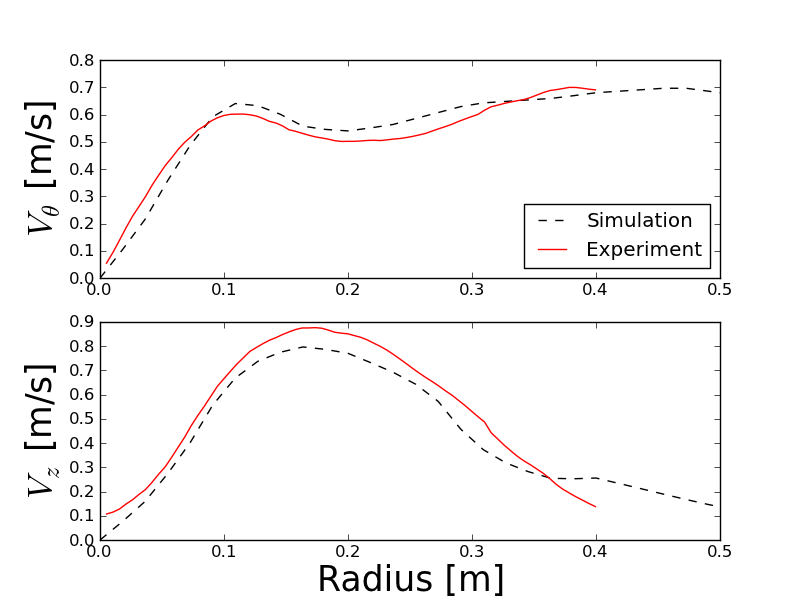
\includegraphics[width = 12 cm]{figs/hybrid_profile}
     \caption{Azimuthal and vertical velocity profiles as a function of
     radius. The simulation and experimental data broadly agree, with
     the simulation also exhibiting the characteristic ``twin-peak''
     structure of the hybrid vanes in the azimuthal velocity. }
     \label{fig:lab}
    \end{center}
  \end{figure}

Figure \ref{fig:lab} is a direct comparisons between laboratory measurements for a simple 
two tier configuration ($55^{\circ}$ top, $30^{\circ}$ bottom)\todo{add gridded vanes} and 
a nominally identical simulation. The simulation and experiment broadly agree. The simulation 
correctly reproduces the twin peak structure in the azimuthal velocity 
observed for this configuration in the experiment. The radial location of peak vertical velocity also 
closely agrees with experiment. The largest observed difference is near the center, where the simulation predicts 
a downward vertical velocity, in contrast to the modest vertical flows measured in the laboratory. 

Similar validation comparisons have been made between several other configurations, notably the $30^{\circ}$ 
and $60^{\circ}$ singly tier straight vane cases, with similar levels of agreement. 
This represents the totality of quantitiative data available for comparison. Qualitative comparisons have been made
between the our simulation results with a mean velocity and with wind tunnel pictures. These images showed
roughly consistent structure between simulation and experiment. Finally. estimates of the energy fluxes between
the field configuration and our simulation results agreed within 15\%. These validation studies have provided a modest 
level of confidence that our simulations accurately reproduce the dynamics observed in real 
vane configurations.\todo{incomplete}

%
% validation story is incomplete
% 
% you have done: 
%
% 1) comparions between laboratory + gridded + virtual 
% 
% 2) comparisons between gridded + virtual in laboratory
%    + field configurations, thermal only and wind
%
% 3) comparisons of virtual vanes to field observations 
%    quantitative + qualitative
%
%
% You need to discuss what needs to be validated -- the
% compare to gridded vanes is a useful validation tool 
%


%
% turbine (explain why we dont need to do it)
%

%% Another significant validation challenge is in modeling the
%% turbines. This is in essence a new embedded 
%% submodel that we will add after validation of the initial configuration
%% is completed. 
